\section{Линеарна регресија}

\subsection{Линеарна регресија со една променлива}
Ова е имплементација на алгоритам за линеарна регресија кој го предвидува
профитот на камион кој превезува храна. Да предпоставиме дека вие сте извршен
директор на ланец ресторани и сакате да го проширите вашиот ланец во некој
друг град. Во ланецот веќе имате камиони во многу различни градови и имате
податоци за профитот и популацијата во тие градови. 

Сакате со помош на овие податоци да добиете помош кој да биде следниот ваш град
во кој ќе се проширите.

Во датотеката population\_profit.txt се наоѓа податочното множество за проблемот
на линеарна регресија. Во првата колона е популацијата на градот, а во втората е
профитот на камионот во тој град. Негативна вредност на профитот значи загуба.

\subsubsection{Исцртување на податоците}

Пред да се започне со било која обработка, вообичаено е корисно да се разберат
податоците со помош на визуелизација. За да ги визуелизираме овие податоци
користиме scatter plot, поради тоа што има само две својства кои се прикажуваат
(профит и популација).


\lstinputlisting[firstline=6,lastline=8,caption=Вчитување на податоците во променливите $X$ и $y$.
]{src/linearRegression/linearRegression.m}


\lstinputlisting[firstline=6,lastline=10,caption=Исцртување на податоците]{src/linearRegression/plotData.m}


\begin{figure}[htb]
\centering
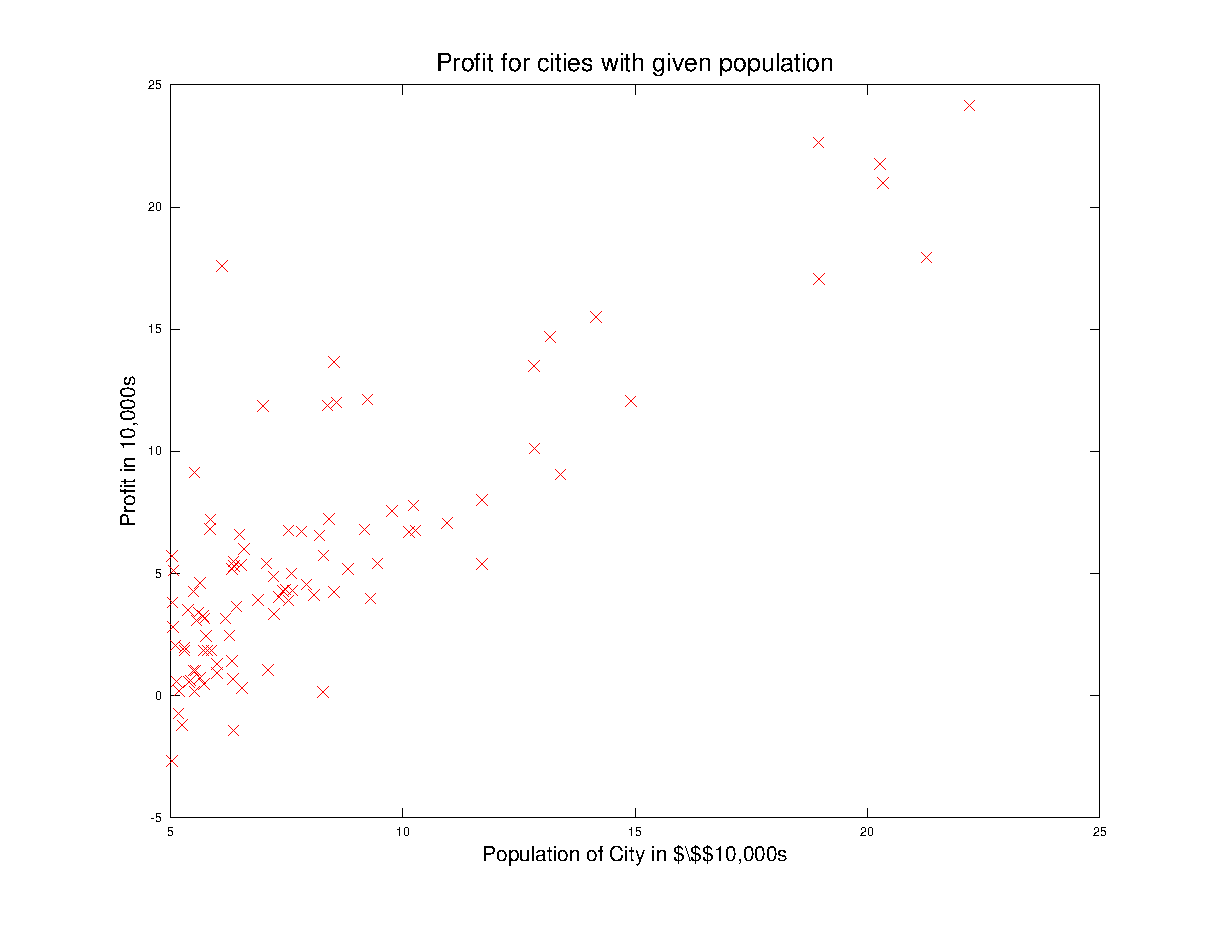
\includegraphics[width=.9\textwidth]{src/linearRegression/data}
\caption{Scatter plot на податочното множество}
\label{fig:plot}
\end{figure}

\subsubsection{Пресметување со Gradient Descent}

Следува имплементација на одредување на параметарот $\theta$ од лиенарната
регресија на податочното множество со помош на gradient descent.

\subsubsection{Равенки за пресметување}

Целта на линеарната регресија е да ја минимизира функцијата на чинење

\[
	J(\theta) = \frac{1}{2m}\sum^m_{i=1}{(h_\theta(x^{(i)}) - y^{(i)})^2}
\]
каде што хипотезата $h_\theta(x)$ е дадена со линеарниот модел:
\[
	h_\theta(x) = \theta^Tx = \theta_0 + \theta_1x_1
\]

Параметрите на моделот се вредностите $\theta_j$.
Алгоритмот го имплементираме со тоа што во секоја итерација ја извршуваме
следата формула:
\[
	\theta_j := \theta_j - \alpha\frac{1}{m}\sum^m_{i=1}{(h_\theta(x^{(i)}) -
	y^{(i)}) x_j}
\]
\emph{Симултано ги менуваме вредностите на $\theta_j$ за секое $j$.}

\subsubsection{Имплементација}

\lstinputlisting[firstline=23,lastline=28,caption=Додавање на дополнителна
колона $\theta_0$ и иницијализција на параметрите.]{src/linearRegression/linearRegression.m}

\subsubsection{Пресметување на функцијата на чинење $J(\theta)$}

\lstinputlisting[firstline=6,lastline=12,caption=Имплементација на
$J(\theta)$]{src/linearRegression/computeCost.m}

\subsubsection{Gradient Descent}

\lstinputlisting[firstline=6,lastline=16,caption=Имплементација
на Gradient Descent]{src/linearRegression/gradientDescent.m}

\begin{figure}[htb]
\centering
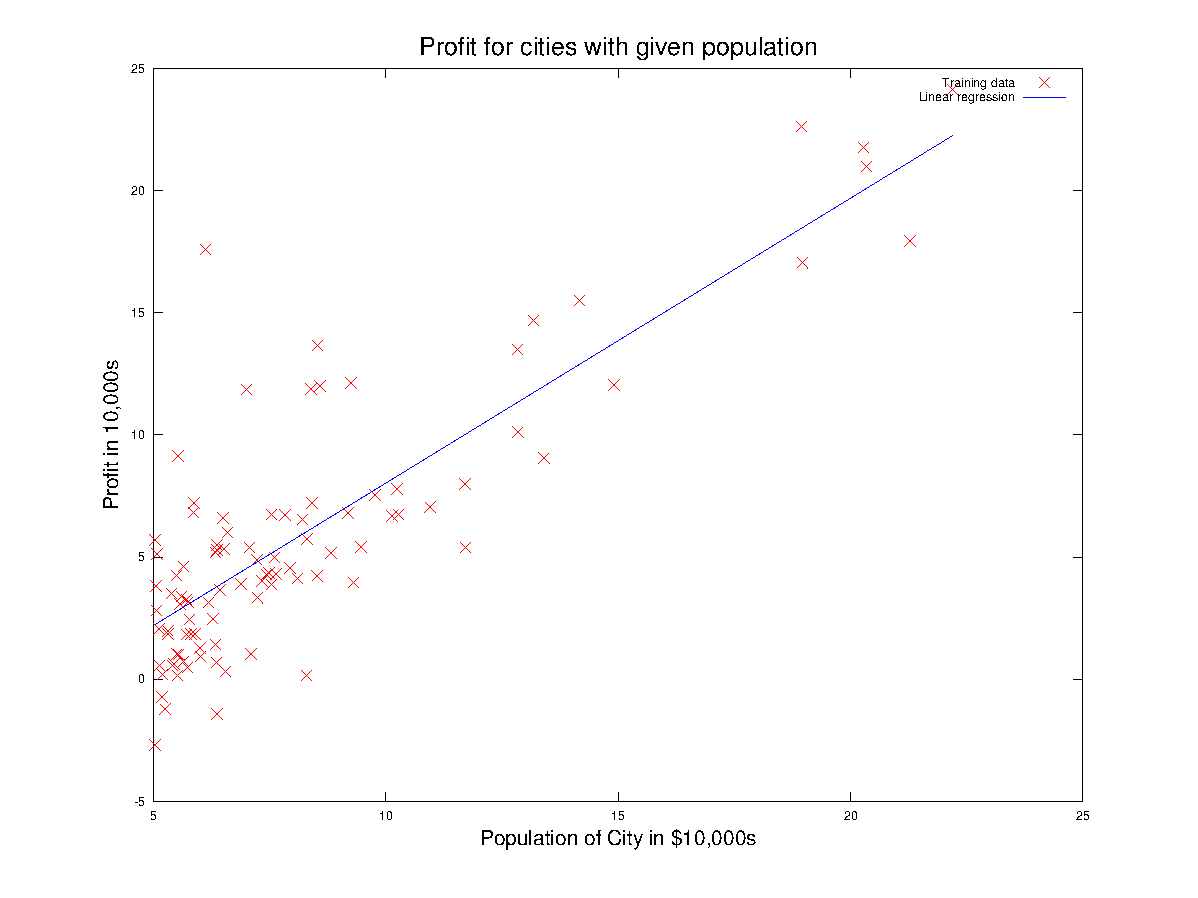
\includegraphics[width=.9\textwidth]{src/linearRegression/line_fit}
\caption{Линеарна регресија на тренинг множеството}
\label{fig:linear_fit}
\end{figure}

\subsubsection{Визуелизација на $J(\theta)$}
За подобро согледување на вредностите на функцијата на чинење $J(\theta)$ ги
исцртуваме нејзините вредност на 2-димензионален грид од вредностите
на $\theta_0$ и $\theta_1$.

Целта на овие графици е да покажат како $J(\theta)$ се менува со менувањето на
$\theta_0$ и $\theta_1$. Функцијата на чинење $J(\theta)$ е обликувана како
вдлабнат сад и има глобален минимум. Ова најубаво се воочува на површинскиот
график во 3Д. Минимумот е оптималната точка за $\theta_0$ и $\theta_1$, со што
алгоритмот gradient descent во секој чекор се доближува поблиску до оваа точка.


\begin{figure}[htbp]
        \begin{subfigure}[b]{0.5\textwidth}
                \centering
                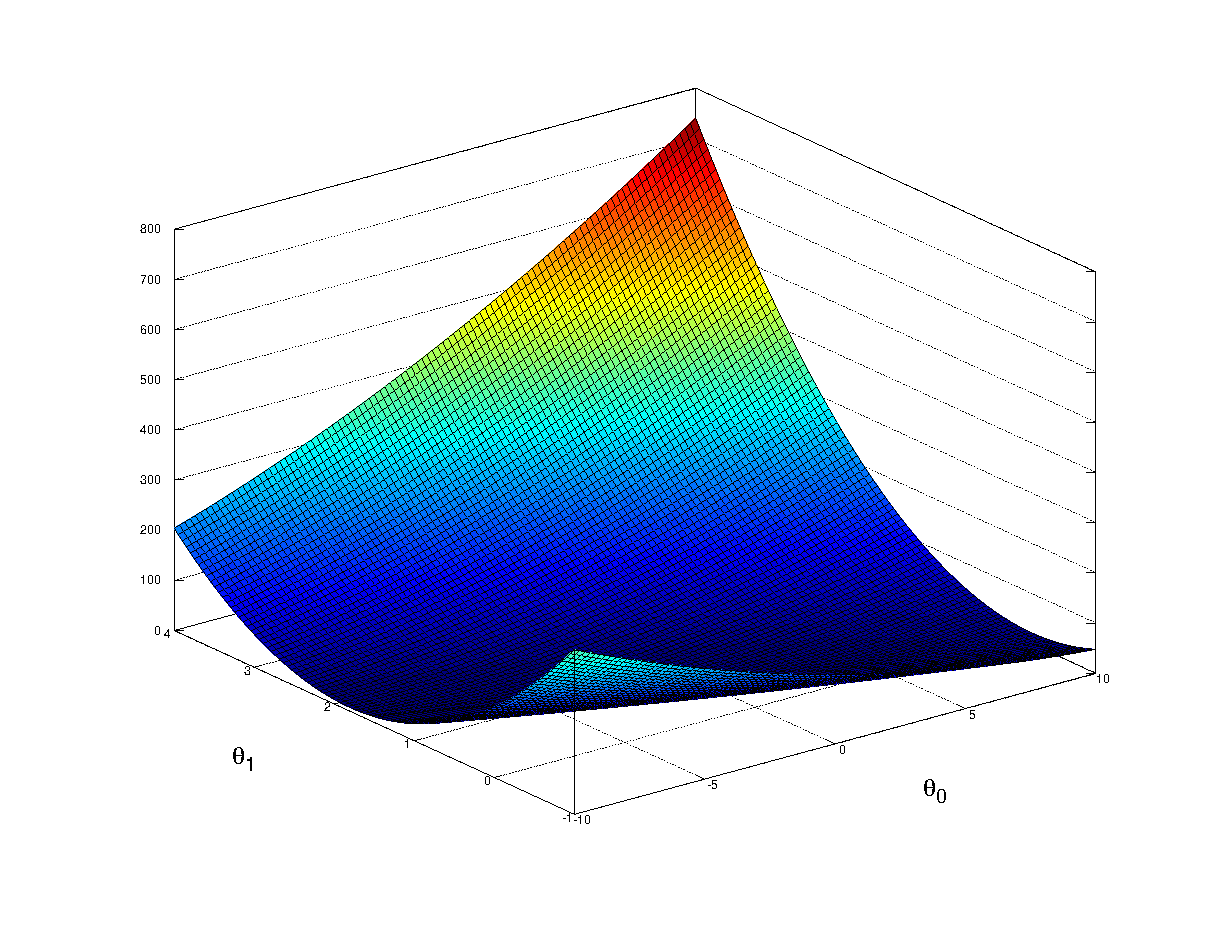
\includegraphics[width=\textwidth]{src/linearRegression/surface_plot}
                \caption{Површина}
                \label{fig:surface}
        \end{subfigure}%
        ~ 
        \begin{subfigure}[b]{0.5\textwidth}
                \centering
                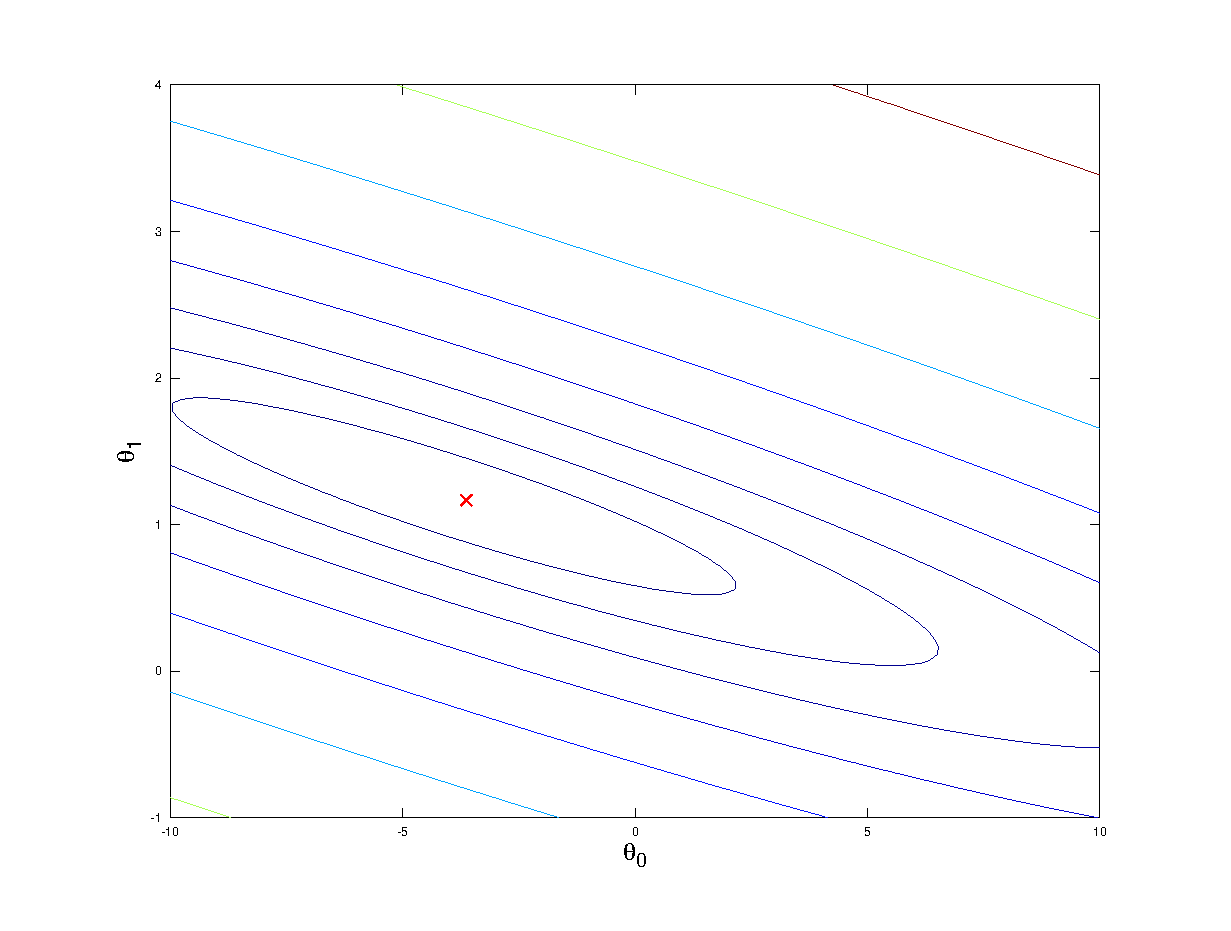
\includegraphics[width=\textwidth]{src/linearRegression/contour}
                \caption{Контура која го прикажува минимумот}
                \label{fig:contour}
        \end{subfigure}
        \caption{Функцијата на чинење $J(\theta)$}
        \label{fig:cost_function}
\end{figure}

\subsection{Линеарна регресија со повеќе променливи}

Со помош на линеарна регресија со повеќе променливи ќе ја предвидуваме цената на
куќите. Да претпоставиме дека продаваме куќа и сакаме да дознаеме која е
нејзината цена на пазарот. Еден начин да го дознаеме ова е да собереме
информации за цените на последно продадените куќи ид да изградиме модел на
цените на куќите.

Во датотеката houses\_prices.txt се содржи податочно множество со цените на
куќите во Портланд, Орегон. Првата колона е големината на куќата (во квадратни
стапки), втората колона е бројот на соби, а третата колона е цената на куќата.

\subsubsection{Нормализација на обележјата}

Помеѓу вредностите на некои обележја постојат многу големи разлики и тоа не е
добро за алгоритмите за машинско учење. Затоа кога постојат вакви огромни
разлики, вредностите на обележјата се нормализираат (скалираат) со што
алгоритмот gradient descent многу побрзо конвергира. 

Нормализацијата ја извршуваме со следните чекори:
\begin{itemize}
  \item Ја одземаме средната вредност од секое обележје во податочното
  множество,
  \item Ги скалираме (делиме) вредностите на обележјата со нивните соодветни
  стандардни девијации.
\end{itemize}

\lstinputlisting[firstline=8,lastline=16,caption=Нормализација
на обележјата]{src/linearRegression/featureNormalize.m}


\subsubsection{Gradient Descent}

\lstinputlisting[firstline=6,lastline=18,caption=Имплементација
на Gradient Descent за повеќе
променливи]{src/linearRegression/gradientDescentMulti.m}


\subsubsection{Нормални равенки}
Точното решение на линеарна регресија може да се определи со равенката:

\[
	\theta = (X^TX)^{-1}X^T\vec{y}.
\]

За да се употребува оваа формула не е потребно скалирање на обележјата и ќе се
добие точно решение во една пресметка: нема „циклус до конвергенција“ како во
претходниот алгоритам.

